\chapter{Experiments}
\label{experiments}
This chapter covers the different experiments conducted in the context of this project. In Section \ref{experiments_table_detection}, we present two experiments on table detection, which investigate the ability of image segmentation models to learn under challenging data condition. Two experiments on table classification are also presented in Section \ref{experiments_table_classification}, where we examine the predictive power of state-of-the-art classifiers using different data modalities on manually and automatically constructed datasets. Finally, in Section \ref{end_to_end}, we present an inconclusive experiment conducted at the beginning of this project that shows the difficulty for image segmentation models to simultaneously solve the tasks of table detection and table classification.

\section{Table detection}
\label{experiments_table_detection}
In Section \ref{table_detection_experiment1}, the performances of dhSegment and Mask R-CNN are compared on datasets with different levels of inconsistencies. In Section \ref{table_detection_experiment2}, these models are compared on a reduced but supposedly perfect dataset.

\subsection{Assessment of a data filtering strategy}
\label{table_detection_experiment1}
Having high quality data is essential to the optimal learning of any machine learning models, but what if the only data available is not? In this experiment, we assess the usefulness of the filtering strategy described in \ref{annotation_survey} -- where problematic clusters are manually identified and removed -- from which \textbf{NLL-filtered} was created out of \textbf{NLL}. Since both datasets are known for being inconsistent, a question that is naturally brought up is whether or not the chosen models are able to learn despite this. To answer it, dhSegment and Mask R-CNN are trained on the two aforementioned datasets and their performances compared on manually constructed datasets.\\
This experiment also serves the purpose of establishing whether object instance image segmentation algorithms are capable of performing semantic image segmentation efficiently, as touched in \ref{table_detection_evaluation}.

\subsubsection{Training}
Models are trained using two different setups summarized in Tables \ref{setup1} and \ref{setup2}. In the first setup, models are trained on \textbf{NLL} using 70\% of the pages for training and 20\% for validation. They are then tested on the remaining 10\%, on \textbf{RB} and on \textbf{NLL-revised}. The second setup is very similar, but models are instead trained (and tested) on \textbf{NLL-filtered} following the same splits.\\
Note that for both setups, \textbf{NLL-revised} only contains pages that are part of the testing splits of \textbf{NLL} and \textbf{NLL-filtered} which ensures that models have not seen these test examples during their training. Finally, we recall that \textbf{RB} has not been annotated at the instance-level, so its evaluation by object instance segmentation metrics should be poor.\\
The different hyper-parameters used for training each model are introduced below. Their search was done by trial and error; they may not lead to the lowest training times but should ensure convergence. This is also the case for the next experiment.

dhSegment and Mask R-CNN were both trained similarly. Their training was done with a batch size of 2 for 25 epochs using batch normalization on a NVIDIA GeForce GTX TITAN X 12GB. An Adam optimizer with an initial learning rate of $10^{-4}$ coupled with a per-epoch exponentially decaying learning rate $\gamma=0.85$ and a L2-regularizer of $10^{-6}$ were used. Both models were pre-trained on the ImageNet dataset. The only difference between both models is their metric to optimize on the validation set, which is the mIoU or dhSegment and the mask segmentation mAP for Mask R-CNN. \\
During training, images are resized to reach an height of 1333 pixels and a width of 800 pixels. After that they are uniformly scaled by a factor randomly sampled from [0.9, 1.1]; the images are cropped to maintain their size. Then, they are slightly rotated 50\% of the time by a degree sampled uniformly from [-1, 1].  \\

For both models, only one run was performed as the training time is very long: about three days for dhSegment, and about two days for Mask R-CNN.

\begin{table}[htp]
\begin{center}
\begin{tabular}{c|c|c||c}
 & Training & Validation & Testing \\
\hline
\textbf{NLL} & \begin{tabular}{@{}c@{}}40,435 tables \\ 19,947 pages (70\%)\end{tabular} &  \begin{tabular}{@{}c@{}}11,706 tables \\ 5,700 pages (20\%)\end{tabular} & \begin{tabular}{@{}c@{}}5,866 tables \\ 2,849 pages (10\%)\end{tabular}\\
\hline
\textbf{RB} &  &  & \begin{tabular}{@{}c@{}}800 tables \\ 474 pages (100\%)\end{tabular}\\
\hline
\textbf{NLL-revised} &  &  & \begin{tabular}{@{}c@{}}5,445 tables \\ 1,500 pages (100\%)\end{tabular}\\
\hline
\end{tabular}
\end{center}
\caption{Table detection, setup 1: datasets splits.}
\label{setup1}
\end{table}%

\begin{table}[htp]
\begin{center}
\begin{tabular}{c|c|c||c}
 & Training & Validation & Testing \\
\hline
\textbf{NLL-filtered} & \begin{tabular}{@{}c@{}}19,641 tables \\ 11,890 pages (70\%)\end{tabular} &  \begin{tabular}{@{}c@{}}5,640 tables \\ 3,399 pages (20\%)\end{tabular} & \begin{tabular}{@{}c@{}}2,813 tables \\ 1,698 pages (10\%)\end{tabular}\\
\hline
\textbf{RB} &  &  & \begin{tabular}{@{}c@{}}800 tables \\ 474 pages (100\%)\end{tabular}\\
\hline
\textbf{NLL-revised} &  &  & \begin{tabular}{@{}c@{}}5,445 tables \\ 1,500 pages (100\%)\end{tabular}\\
\hline
\end{tabular}
\end{center}
\caption{Table detection, setup 2: datasets splits.}
\label{setup2}
\end{table}%

\subsubsection{Results}
Results for the first setup, where models are trained on the large but highly inconsistent \textbf{NLL}, are shown in Table \ref{setup1_results}, while results for the second setup, where models are trained on the medium-sized but mildly inconsistent \textbf{NLL-filtered}, are shown in Table \ref{setup2_results}. \\
In both setups, when evaluated on \textbf{NLL-revised}, Mask R-CNN outperforms dhSegment on all metrics. This means that Mask R-CNN is better than dhSegment at semantically detecting tables on newspaper pages when trained with inconsistent data. We believe that this may be due in part to the fact that Mask R-CNN considers every predictions with a confidence score greater than 0.05 it makes. This means that even if Mask R-CNN thinks a Region of Interest has only 5\% chance of being a table, it will be part of its prediction. As in most object instance image segmentation algorithms, low-certainty predictions are not discarded assuming that they can be filtered later based on the overall Precision-Recall ratio one is interested in. This explanation seems to be corroborated by \citet{wenkel_confidence_2021} who state that, in the context of object detection algorithms, ``most neural networks use a rather low threshold as a high number of false positives is not penalized by standard evaluation metrics''. Indeed, this strategy would therefore not be penalized on \textbf{NLL-revised} since it contains many more tables than \textbf{NLL}. False positives in the latter dataset appear to result in true positives in the former. The large APs of Mask R-CNN on both \textbf{NLL} and \textbf{NLL-filtered} also point in that direction, as the model is perfectly capable of performing well on a testing dataset representative of its training: a large number of false positives is indeed not penalized by standard evaluation metrics for object detection.  \\
Looking at the results of both models for both setups on the test sets of the data they were trained with, we find that dhSegment generally outperforms Mask R-CNN on all metrics except mIoU and R@50:5:95 for \textbf{NLL}. We should also point out the notable increase in mIoU for dhSegment between both datasets when trained with the more consistent dataset \textbf{NLL-filtered} compared to \textbf{NLL}. Overall, this suggests that dhSegment is better than Mask R-CNN when tested on data representative of that on which it was trained on, and that when the data is more consistent, it is able to achieve better performance on semantic segmentation metrics. It is true that Mask R-CNN also sees a performance increase on the mIoU, but it is smaller than that of dhSegment (+0.48 vs +1.65 on the mIoU). We can therefore conclude that the filtering strategy is favorable to dhSegment. Indeed, its performance in terms of mIoU on \textbf{NLL-revised} increases by 5.82 between the two setups, while those of Mask R-CNN decrease by 1.05. Mask R-CNN suffered from the filtering strategy; because of it, it was subjected to less tables, and even if these are known to be inconsistently labelled, Mask R-CNN is able to learn from them. This is also confirmed by its APs which decrease by 0.35 between both setups. \\
In both setups, for dhSegment, we notice a large drop in Precision between the \textbf{NLL} and \textbf{NLL-filtered} test sets and \textbf{NLL-revised}, but a small drop in Recall. Since both \textbf{NLL} and \textbf{NLL-filtered} test sets lack some tables in their ground truth compared to \textbf{NLL-revised}, it is more difficult for the models to reach the IoU threshold that will turn a prediction into a true positive instead of a false positive. As a result, the number of false positives increases and the number of true positives decreases, greatly reducing the Precision. Concerning the Recall, both test sets contain tables that incorrectly labelled as such, which is not the case in \textbf{NLL-revised}. It is likely that dhSegment correctly guessed that certain tables were actually not tables, which was initially penalized due to erroneous ground truth in the test sets but encouraged in \textbf{NLL-revised}. As a result, the number of false negatives decreased, which had less of an impact on the overall decrease in Recall.\\
For \textbf{RB}, we again see a clear advantage on non-representative datasets for Mask R-CNN on all metrics. Also noteworthy are the extremely low AP scores for Mask R-CNN, showing the price to be paid when using consistently annotated ground truths at too coarse a granularity. Mask R-CNN is unable to understand what an instance of a table is and scores terribly. Finally, the same point can be made about the APs on \textbf{NLL-revised} which shows that the inconsistent granularity of the annotations of \textbf{NLL} severely hinders the performance of this object instance detection model on a dataset it should excel. \\
In summary, both models are capable of learning with inconsistent data, as their results on correctly labelled data are encouraging, especially for Mask R-CNN, showing that object instance segmentation algorithms are very well suited for semantic segmentation. So much so that they can even outperform models that were designed specifically for this task in a context of inconsistent training data. Finally, concerning the filtering strategy, we saw that it mainly favors dhSegment as Mask R-CNN sees a generalized decrease in its performance. 

%TODO example of same prediction of Mask on NLL NLL-filtered and NLL-revised and semantically

\begin{table}[htp]
\begin{center}
\begin{tabular}{cc|c|c|c}
Metric & Models & NLL & RB & NLL-revised \\
\hline
mIoU & dhSegment & 80.02 & 62.03 & 70.75\\
 & Mask R-CNN &  \textbf{80.23} &  \textbf{67.94} &  \textbf{83.19}\\
 \hline
P@60 & dhSegment &  \textbf{86.75} & 66.67 & 75.26\\
 & Mask R-CNN & 84.55 &  \textbf{73.85} &  \textbf{90.13}\\
  \hline
R@60 & dhSegment &  \textbf{96.82} & 91.69 & 94.38\\
 & Mask R-CNN & 96.78 &  \textbf{94.65} &  \textbf{98.11}\\
  \hline
P@80 & dhSegment &  \textbf{74.66} & 36.47 & 53.26\\
 & Mask R-CNN & 70.08 &  \textbf{43.08} &  \textbf{71.02}\\
 \hline
R@80 & dhSegment &  \textbf{96.32} & 85.79 & 92.23\\
 & Mask R-CNN & 96.14 &  \textbf{91.16} &  \textbf{97.61}\\
 \hline
 P@50:5:95 & dhSegment &  \textbf{74.06} & 45.19 & 59.01\\
 & Mask R-CNN & 73.25 &  \textbf{50.15} &  \textbf{75.24}\\
 \hline
 R@50:5:95 & dhSegment & 95.89 & 78.99 & 91.98\\
 & Mask R-CNN &  \textbf{96.16} &  \textbf{84.45} &  \textbf{97.60}\\
 \hline
  \hline
 AP@50:5:95 & Mask R-CNN & 0.815 & 0.128  & 0.593\\
  \hline
\end{tabular}
\end{center}
\caption{Table detection, setup 1: results.}
\medskip
\small
dhSegment and Mask R-CNN have been trained on \textbf{NLL}, the results presented here correspond to their evaluation on an unseen testing split of \textbf{NLL}, \textbf{RB} and \textbf{NLL-revised}.
\label{setup1_results}
\end{table}%

\begin{table}[htp]
\begin{center}
\begin{tabular}{cc|c|c|c}
Metric & Models & NLL-filtered & RB & NLL-revised \\
\hline
mIoU & dhSegment & \textbf{81.67} & 59.01 & 76.57 \\
 & Mask R-CNN & 80.71 & \textbf{71.09} & \textbf{82.14}\\
 \hline
P@60 & dhSegment & \textbf{89.04} & 61.23 & 86.83\\
 & Mask R-CNN & 87.17 & \textbf{74.36} & \textbf{91.81}\\
  \hline
R@60 & dhSegment & \textbf{96.97} & 93.29 & 94.87\\
 & Mask R-CNN & 95.36 & \textbf{98.31} & \textbf{97.86}\\
  \hline
P@80 & dhSegment & \textbf{78.51} & 27.09 & 61.81\\
 & Mask R-CNN & 76.37 & \textbf{48.93} & \textbf{68.42}\\
 \hline
R@80 & dhSegment & \textbf{96.57} & 86.01 & 92.94\\
 & Mask R-CNN & 94.74 & \textbf{97.45} & \textbf{97.14}\\
 \hline
P@50:5:95 & dhSegment & \textbf{76.91} & 38.63 & 67.81\\
 & Mask R-CNN & 76.46 & \textbf{53.08} & \textbf{73.64}\\
 \hline
R@50:5:95 & dhSegment & \textbf{96.14} & 76.81 & 92.29\\
 & Mask R-CNN & 94.50 & \textbf{95.06} & \textbf{97.09}\\
 \hline
  \hline
 AP@50:5:95 & Mask R-CNN & 0.806 & 0.131 & 0.558\\
  \hline
\end{tabular}
\end{center}
\caption{Table detection, setup 2: results.}
\medskip
\small
dhSegment and Mask R-CNN have been trained on \textbf{NLL-filtered}, the results presented here correspond to their evaluation on an unseen testing split of \textbf{NLL-filtered}, \textbf{RB} and \textbf{NLL-revised}.
\label{setup2_results}
\end{table}%

\subsection{Reducing the amount of training data}
\label{table_detection_experiment2}
In this experiment, the following question is addressed: are visual models capable of detecting tables in newspaper with very few training material? It also aims to provide some answers to another question: should efforts be aimed at manually annotating a small but perfect dataset, at (semi-)automatically correcting an inconsistent but large dataset or simply at gathering more training material? \\
dhSegment and Mask R-CNN are here trained on \textbf{NLL-revised}, a small and manually annotated at the instance-level. The latter property allows a proper comparison between both models as the training material is (contrary to the previous experiment) perfectly adapted for both segmentation paradigms.

\subsubsection{Training}
Both models are trained following the setup described in Table \ref{setup3}. 80\% of \textbf{NLL-revised} is used to train and validate the models, and 20\% is used to test them. Because of the small size of the dataset, it is necessary to reserve a larger split for testing than in the previous experiment in order to cover sufficiently many different cases. \\
dhSegment and Mask R-CNN were trained similarly to the previous experiment, the only differences being the number of epochs of 100, and $\gamma=0.95$.\\

Again, a single run was performed for both models, with dhSegment taking nearly two days to train, while Mask R-CNN took about a day and a half.

\begin{table}[htp]
\begin{center}
\begin{tabular}{c|c|c||c}
 & Training & Validation & Testing \\
\hline
\textbf{NLL-revised} & \begin{tabular}{@{}c@{}}3412 tables \\ 900 pages (60\%)\end{tabular} &  \begin{tabular}{@{}c@{}}985 tables \\ 300 pages (20\%)\end{tabular} & \begin{tabular}{@{}c@{}}1048 tables \\ 300 pages (20\%)\end{tabular}\\
\hline
\end{tabular}
\end{center}
\caption{Table detection, setup 3: dataset splits.}
\label{setup3}
\end{table}%

\subsubsection{Results}
The results of this experiment are presented in Table \ref{setup3_results}. It can be seen that consistent manual annotation efforts pay off, as both models perform very well for all metrics. dhSegment clearly outperforms Mask R-CNN in terms of mIoU and Precision, but performs slightly worse in terms of Recall. Mask R-CNN is better in the latter metric for the reason mentioned in the previous experiment, where it produces a lot of predictions, thus increasing Recall. In fact, both models perform very well on metrics directly associated with their segmentation strategies, which means that dhSegment performs very well in terms of mIoU and Mask R-CNN in terms of AP. This indicates that having very little but qualitative data may be enough for these models to accurately learn what a table is. However, they would need to be tested on a different, non-representative dataset for this to be affirmed. 

\begin{table}[htp]
\begin{center}
\begin{tabular}{cc|c}
Metric & Models & NLL-revised \\
\hline
mIoU & dhSegment & \textbf{84.10} \\
 & Mask R-CNN & 81.00\\
 \hline
P@60 & dhSegment & \textbf{93.15}\\
 & Mask R-CNN & 87.71\\
  \hline
R@60 & dhSegment & 98.91\\
 & Mask R-CNN & \textbf{99.23}\\
  \hline
P@80 & dhSegment & \textbf{81.51}\\
 & Mask R-CNN & 67.58\\
 \hline
R@80 & dhSegment & 98.76\\
 & Mask R-CNN & \textbf{99.00}\\
 \hline
P@50:5:95 & dhSegment & \textbf{76.47} \\
 & Mask R-CNN & 70.17 \\
 \hline
R@50:5:95 & dhSegment & 98.09\\
 & Mask R-CNN & \textbf{98.82} \\
 \hline
 \hline
 AP@50:5:95 & Mask R-CNN & 0.763 \\
  \hline
\end{tabular}
\end{center}
\caption{Table detection, setup 3: results.}
\medskip
\small
dhSegment and Mask R-CNN have been trained on \textbf{NLL-revised}, the results presented here correspond to their evaluation on an unseen testing split of \textbf{NLL-revised}.
\label{setup3_results}
\end{table}%

\subsection{Summary and discussion}
These two experiments show that the task of table detection can be successfully addressed by both dhSegment and Mask R-CNN. In terms of semantic segmentation in a context of inconsistent data, Mask R-CNN has the upper hand due to its non-conservative prediction strategy. However, when the data is correctly labelled dhSegment shows better results. This means that dhSegment shines on test data representative of the data it was trained on, while Mask R-CNN is able to provide better transferability. \\
In terms of object instance segmentation, dhSegment is inherently unable to provide a solution, while Mask R-CNN can only provide good results if the training data is of good quality. If tables need to be classified later, then it seems that the most viable strategy is to use Mask R-CNN and quality data to perform accurate object instance detection. Indeed, table classification makes no sense if classifiers are given segmentation masks containing multiple tables, so semantic segmentation should be avoided in that regard. Now, if we only wish to know the regions of the newspaper pages where tables lie in order to, for example, remove these regions from the OCR processing, the decision as to which model is best is not as clear-cut. It all comes down to whether or not the effort of collecting quality data is worth the additional performance that dhSegment can provide over Mask R-CNN with poorly annotated data.

\section{Table classification}
\label{experiments_table_classification}
In Section \ref{classification_benchmark}, the performances of RoBERTa, LayoutLM (without making use of the visual modality) and LayoutXLM are compared on a classification task. In Section \ref{auto_tag}, the benefits of using an automatically augmented dataset are assessed based on the results of these three models.

\subsection{Data modality comparison}
\label{classification_benchmark}
Using different data modalities in a model is costly in terms of acquisition, retrieval and computation. \textit{impresso}'s pipeline provides easy access to the image files and OCR output from its entire newspaper collection; however, its OCR text output is known to be messy in regions where tables are located, and images are heavy objects to process. In this context, a question arises: is the text provided by the OCR sufficient to effectively classify the tables, and if not, is the addition of other data modalities useful enough to justify the use of heavier models and higher data throughputs? \\
In this experiment, three data modalities are used and compared: i) the OCR text output; ii) the bounding box coordinates of each word detected by OCR; iii) the image regions of these words. RoBERTa (text), LayoutLM (text + layout) and LayoutXLM (text + layout + image) are compared on a manually labelled dataset to evaluate the contribution of each modality.

\subsubsection{Training}
The three models are trained and tested according to the setup shown in Table \ref{data_modality_setup}. \textbf{NLL-tag} is divided into training, validation and testing sets following a 60\%/20\%/20\% distribution in terms of page count. The split was done by stratified sampling on the table labels to get similar class distributions on the sets to ensure good training and fair testing.  \\
The three models were trained for 10 epochs with a batch size of 4, following the default hyper-parameters of the implementation used, as explained in \ref{table_classification}. \\

RoBERTa and LayoutLM took around an hour to train, while LayoutXLM took around 3 hours. Only one run is reported for all models. 

\begin{table}[htp]
\begin{center}
\begin{tabular}{wr{3cm}||c|c|c}
 & Training & Validation & Testing \\
Class & \begin{tabular}{@{}wl{2cm}wr{1cm}@{}}Tables & Pages \end{tabular}& \begin{tabular}{@{}wl{2cm}wr{1cm}@{}}Tables & Pages \end{tabular}& \begin{tabular}{@{}wl{2cm}wr{1cm}@{}}Tables & Pages \end{tabular}\\
\hline
\begin{tabular}{@{}wr{3cm}@{}}exchange (E) \\ food prices (F)  \\ miscellaneous (M) \\ sport results (S) \\ transport schedules (T) \\ weather (W) \end{tabular} & \begin{tabular}{@{}wl{2cm}wr{1cm}@{}}265 (11.3\%)& 188\\ 108  (4.6\%) & 86\\276 (11.7\%) & 145\\238 (10.1\%) & 25\\1,452 (61.7\%) & 245\\15  (0.6\%) & 14\end{tabular} & \begin{tabular}{@{}wl{2cm}wr{1cm}@{}} 79 (14.4\%) & 55 \\ 30 (5.5\%) & 28  \\ 82 (14.9\%) & 48 \\ 37 (6.7\%) & 7 \\ 318 (57.9\%) & 68 \\ 3 (0.5\%) & 3 \end{tabular} &  \begin{tabular}{@{}wl{2cm}wr{1cm}@{}}100 (11.4\%) & 69 \\ 39 (4.4\%) & 29  \\ 71 (8.1\%) & 44 \\ 128 (14.5\%) & 9 \\ 531 (60.3\%) & 95\\ 11 (1.3\%) & 11  \end{tabular}\\
\hline
\begin{tabular}{@{}wr{3cm}@{}} Total \\ Percentage\end{tabular} & \begin{tabular}{@{}wl{2cm}wr{1cm}@{}}2,354 & 605 \\ 62.2\% & 61.5\%\end{tabular} & \begin{tabular}{@{}wl{2cm}wr{1cm}@{}} 549 & 173 \\ 14.5\% & 17.6\%\end{tabular} &  \begin{tabular}{@{}wl{2cm}wr{1cm}@{}}880 & 206 \\ 23.3\% & 20.9\%\end{tabular}\\
\end{tabular}
\end{center}
\caption{Table classification, setup 1: \textbf{NLL-tag} splits.}
\label{data_modality_setup}
\end{table}%

\subsubsection{Results}
The results of this experiment are shown in Table \ref{table_classification_setup1_results}. The picture is quite clear here, with both LayoutLM and LayoutXLM significantly outperforming RoBERTa on all averaged metrics. This shows the contribution of both layout and image modalities. Only adding the layout modality already shows a strong increase in performance, proving that the table structures convey significant signal and is able to strongly compensate for a noisy OCR text output. The addition of a third modality allows LayoutXLM to extract extra signal from these tables, becoming the best of these three classifiers on the averaged metrics. This shows that tables also carry important visual features that are useful in ambiguous cases.\\
Interestingly, RoBERTa outperforms the other two models in terms of Precision on three classes: food prices, miscellaneous and sport results. This shows that these classes have unique semantics. For example, sport results usually contain team or athlete names that will never be found in other classes. In such cases, RoBERTa is able to be extremely precise; however, the associated low recall leads us to believe that this only occurs when the quality of the OCR is good enough to recognize these words. Indeed, looking at Figure \ref{roberta_B1}, we see that RoBERTa almost always confuses sport results with transport schedule. This is most likely due to the fact that sport results often contain some numbers like game scores that could be confused with times in transport schedules. The large imbalance in classes doesn't help either.\\
Overall, the addition of modalities proves to be very useful. However, this comes at the cost of heavier computational loads, especially for the image modality where the gains from its use can be considered as marginal.

\begin{table}[htp]
\begin{center}
\begin{tabular}{cc|cccccc|cc}
Metric & Models & E & F & M & S & T & W & M. avg. & W. avg.  \\
\hline
Precision & RoBERTa & 86.41 & \textbf{94.87} & \textbf{94.73} & \textbf{100.00} & 79.01 & 0.00 & 75.84 & 83.89\\
 & LayoutLM & 94.12 & 83.33 & 88.71 & 98.40 & 98.33 & 90.91 & 92.30 & 96.33  \\
 & LayoutXLM & \textbf{98.91} & 90.00 & 86.30 & 98.41 & \textbf{98.51} & \textbf{100.00} & \textbf{95.36} & \textbf{97.20}  \\
 \hline
Recall & RoBERTa & 89.00 & \textbf{94.87} & 76.06 & 10.94 & 99.25 & 0.00 & 61.69 & 81.93\\
 & LayoutLM & \textbf{96.00} & 89.74 & 77.46 & 96.09 & 99.62 & 90.91 & 91.64 & 96.36  \\
  & LayoutXLM & 91.00 & 92.31 & \textbf{88.73} & \textbf{96.88} & \textbf{99.81} & \textbf{100.00} & \textbf{94.79} & \textbf{97.16}  \\
   \hline
 F1-score & RoBERTa & 87.68 & \textbf{94.87} & 84.37 & 19.72 & 87.98 & 0.00 & 62.44 & 76.93  \\
 & LayoutLM & \textbf{95.05} & 86.42 & 82.71 & 97.23 & 98.97 & 90.91 & 91.88 & 96.30  \\
  & LayoutXLM & 94.79 & 91.14 & \textbf{87.50} & \textbf{97.64} & \textbf{99.16} & \textbf{100.00} & \textbf{95.04} & \textbf{97.16}  \\
   \hline
\end{tabular}
\end{center}
\caption{Table classification, setup 1: results.}
\medskip
\small
RoBERTa, LayoutLM and LayoutXLM were trained on \textbf{NLL-tag} and are here evaluated on an unseen testing split of this dataset. Results for each class are reported: E) exchange; F) food prices; M) miscellaneous; S) sport results; T) transport schedule; W) weather. \\
M. avg. stands for macro average and corresponds to the average of the results of the 6 classes; while W. avg. stands for weighted average and corresponds to the average of the results of the 6 classes weighted by their respective population size.
\label{table_classification_setup1_results}
\end{table}%

\begin{figure}
\centering
\begin{tabular}{ccc}
\subfloat[RoBERTa\label{roberta_B1}]{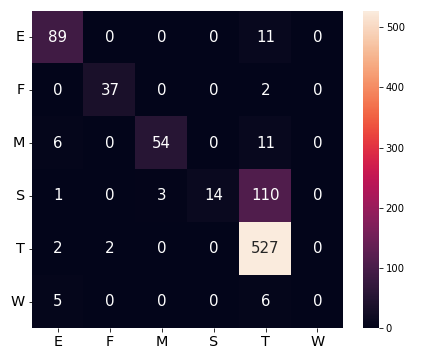
\includegraphics[width=0.3\textwidth]{roberta_B1.png}} &
\subfloat[LayoutLM\label{layoutlm_B1}]{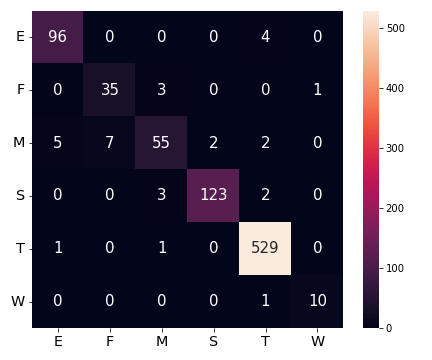
\includegraphics[width=0.3\textwidth]{layoutlm_B1.png}} &
\subfloat[LayoutXLM\label{layoutxlm_B1}]{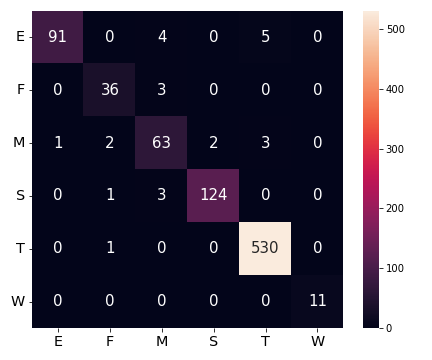
\includegraphics[width=0.3\textwidth]{layoutxlm_B1.png}} \\
\subfloat[RoBERTa\label{roberta_C}]{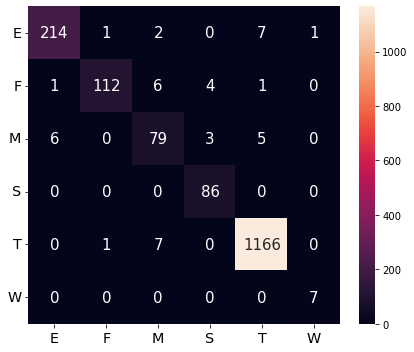
\includegraphics[width=0.3\textwidth]{roberta_C.png}} &
\subfloat[LayoutLM\label{layoutlm_C}]{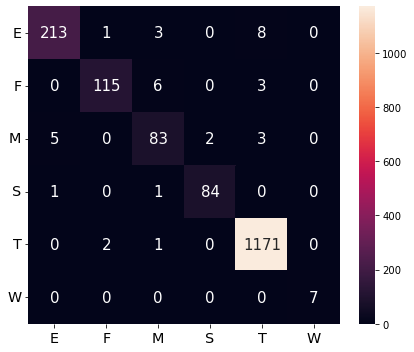
\includegraphics[width=0.3\textwidth]{layoutlm_C.png}} &
\subfloat[LayoutXLM\label{layoutxlm_C}]{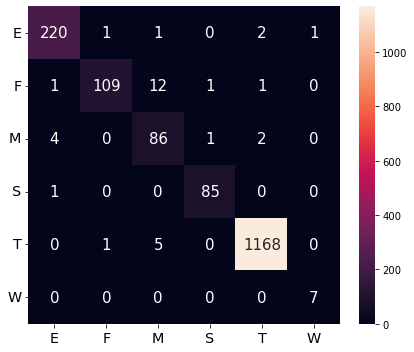
\includegraphics[width=0.3\textwidth]{layoutxlm_C.png}} \\
\end{tabular}
\caption{Confusion matrices for both experiments on table classification.}
\medskip
\small
The first row shows the results of the three classifiers trained on \textbf{NLL-tag}, while the second row shows the results of the three classifiers trained on \textbf{NLL-auto}. Abbrevations are as follows: E) exchange; F) food prices; M) miscellaneous; S) sport results; T) transport schedule; W) weather. 
\label{confusion_matrices}
\end{figure}

\subsection{The benefits of auto-tagging}
\label{auto_tag}
Labelling data is a time-consuming and tedious process necessary for models to learn efficiently. What if this process could be alleviated through automation? This experiment evaluates the suitability of the automatic data augmentation strategy described in \ref{automatic_classification_of_tables}, which automatically labels visually similar tables. Indeed, as explained before, since the OCR output around the tables is noisy, we hope to bring some robustness to classifiers through the textual features of the tables by relying on their more stable visual features.

\subsubsection{Training}
The same three models as in the previous experiment are trained and tested on \textbf{NLL-auto} following the setup defined in Table \ref{auto_tag_setup}. Unlike the previous experiment, the splits are performed here on the table classes, which is motivated by two reasons. First, because the manually labelled tables -- which should make up the entire test set -- originate from a small number of pages due to the way the annotation process was executed, the splits could not be performed properly on the pages as before. Second, this allows for optimal stratified sampling across table classes. Nevertheless, the large difference in pages between the validation and the test splits should be noted as it certainly indicates a lack of variety in terms of newspaper issues in the test set. \\
The models were trained similarly to the previous experiment, i.e. for 10 epochs with a batch size of 4, following the default hyper-parameters of the used implementation. \\

RoBERTa and LayoutLM took around two hours and a half to train, while LayoutXLM took around eight hours. Only one run is reported for all models. 

\begin{table}[htp]
\begin{center}
\begin{tabular}{wr{3cm}||c|c|c}
 & Training & Validation & Testing \\
Class & \begin{tabular}{@{}wl{2cm}wr{1cm}@{}}Tables & Pages \end{tabular}& \begin{tabular}{@{}wl{2cm}wr{1cm}@{}}Tables & Pages \end{tabular}& \begin{tabular}{@{}wl{2cm}wr{1cm}@{}}Tables & Pages \end{tabular}\\
\hline
\begin{tabular}{@{}wr{3cm}@{}}exchange (E)\\ food prices (F)\\ miscellaneous (M) \\ sport results (S) \\ transport schedules (T)\\ weather (W)\end{tabular} & \begin{tabular}{@{}wl{2cm}wr{1cm}@{}}674 (13.2\%)& 569\\ 370 (7.2\%) & 360\\277 (5.4\%) & 186\\257 (5.0\%) & 48\\3,521 (68.8\%) & 2,459\\21 (0.4\%) & 21\end{tabular} & \begin{tabular}{@{}wl{2cm}wr{1cm}@{}} 224 (13.2\%) & 214 \\ 122 (7.2\%) & 120  \\ 91 (5.3\%) & 75 \\ 85 (5.0\%) & 34 \\ 1,173 (68.9\%) & 1,002 \\ 7 (0.4\%) & 7 \end{tabular} &  \begin{tabular}{@{}wl{2cm}wr{1cm}@{}}225 (13.2\%) & 173 \\ 124 (7.3\%) & 104  \\ 93 (5.4\%) & 81 \\ 86 (5.0\%) & 30 \\ 1,174 (68.7\%) & 356\\ 7 (0.4\%) & 7  \end{tabular}\\
\hline
\begin{tabular}{@{}wr{3cm}@{}} Total \\ Percentage\end{tabular} & \begin{tabular}{@{}wl{2cm}wr{1cm}@{}}5,120 & 3,526 \\ 60.0\% & 76.4\%\end{tabular} & \begin{tabular}{@{}wl{2cm}wr{1cm}@{}} 1,702 & 1,451 \\ 20.0\% & 31.4\%\end{tabular} &  \begin{tabular}{@{}wl{2cm}wr{1cm}@{}}1,709 & 684 \\ 20.0\% & 14.8\%\end{tabular}\\
\end{tabular}
\end{center}
\caption{Table classification, setup 2: \textbf{NLL-auto} splits.}
\label{auto_tag_setup}
\end{table}%

\subsubsection{Results}
In Table \ref{table_classification_setup2_results}, the results of this experiment are presented. They are in line with the previous experiment, as the addition of data modalities proves beneficial, with LayoutXLM performing better than the other two models on weighted averaged metrics. We also notice an overall increase in these metrics for all models compared to the previous experiment. This shows that automatically augmenting the dataset is a good strategy. The models are indeed able to achieve better performance by examining more examples. In particular, RoBERTa saw its performance greatly improved compared to the previous experiment.\\
An important point to note is that Precision and Recall across classes are consistent for all models which means that they have built a better intuition for each class with the added examples, besides for the miscellaneous class which proves to be challenging for all three models. This is confirmed by comparing the confusion matrices, in Figure \ref{confusion_matrices}, between the classifiers in the previous experiment and those in this experiment. \\
In short, the automatic labelling strategy paid off as all classifiers saw an increase in performance. Relying on visual similarity to build a stronger sense for each class in terms of the other modalities was the way forward. If we consider the case of LayoutLM which does not have access to visual features (unlike LayoutXLM), we find that its performance is extremely close to LayoutXLM even though it cannot know that the dataset contains clusters of visually similar tables due to the way it was constructed.

\begin{table}[htp]
\begin{center}
\begin{tabular}{cc|cccccc|cc}
Metric & Models & E & F & M & S & T & W & M. avg. & W. avg.   \\
\hline
Precision & RoBERTa & 96.83 & \textbf{98.25} & 84.04 & 92.47 & 98.90 & 87.50 & 93.00 & 97.40\\
 & LayoutLM & 97.26 & 97.46 & \textbf{88.30} & \textbf{99.67} & 98.82 & \textbf{100.00} &  \textbf{96.58} & 97.89  \\
 & LayoutXLM & \textbf{97.35} & 98.20 & 82.69 & 97.70 & \textbf{99.57} & 87.50 & 93.84 & \textbf{98.12}  \\
 \hline
Recall & RoBERTa & 95.11 & 90.32 & 84.95 & \textbf{100.00} & 99.32 & \textbf{100.00} & 94.95 & 97.37\\
 & LayoutLM & 94.67 & \textbf{92.74} & 89.25 & 97.67 & \textbf{99.74} & \textbf{100.00} & 95.68 & 97.89  \\
  & LayoutXLM & \textbf{97.78} & 87.90 & \textbf{92.47} & 98.84 & 99.49 & \textbf{100.00} & \textbf{96.08} & \textbf{98.01}  \\
   \hline
 F1-score & RoBERTa & 95.96 & 94.12 & 84.50 & 96.09 & 99.11 & 93.33 & 93.85 & 97.36\\
 & LayoutLM & 95.95 & \textbf{95.04} & \textbf{88.77} & 97.67 & 99.28 & \textbf{100.00} & \textbf{96.12} & 97.88 \\
  & LayoutXLM & \textbf{97.56} & 92.28 & 87.31 & \textbf{98.27} & \textbf{99.53} & 93.33 & 94.79 & \textbf{98.03}  \\
   \hline
\end{tabular}
\end{center}
\caption{Table classification, setup 2: results.}
\medskip
\small
RoBERTa, LayoutLM and LayoutXLM were trained on \textbf{NLL-auto} and are here evaluated on an unseen testing split of manually labelled tables from this dataset. Results for each class are reported: E) exchange; F) food prices; M) miscellaneous; S) sport results; T) transport schedule; W) weather. \\
M. avg. stands for macro average and corresponds to the average of the results of the 6 classes; while W. avg. stands for weighted average and corresponds to the average of the results of the 6 classes weighted by their respective population size.
\label{table_classification_setup2_results}
\end{table}%

\subsection{Summary and discussion}
These two experiments prove that table classification can be handled very well by state-of-the-art classifiers such as LayoutLM and LayoutXLM. The use of the layout modality proves to be extremely relevant, as it allows LayoutLM to understand that it is dealing with a table without the need for visual features. On a small dataset, the use of the visual modality is well rewarded as LayoutXLM can outperform LayoutLM by a reasonable margin. However, as the size of the dataset increases, this margin decreases significantly. Since the training time of LayoutXLM is about three times that of LayoutLM (without image modality) one may question the need to add this visual modality in production.\\
Finally, we would like to point out that the datasets used for these experiments could be slightly reworked to obtain a more affirmative evaluation. Indeed, the tables to be classified here come from the original segmentation provided by the National Library of Luxembourg, which sometimes includes multiple tables in the same instance. However, we are sure that these tables do not cover different classes. The guidelines followed for the manual annotation were not perfectly established, and we know that some of the items in the dataset are likely not tables. Finally, we believe the models should be tested on a less representative dataset to assess the transferability of these models before putting them into production.

\section{End-to-end: table detection and classification}
\label{end_to_end}
dhSegment and Mask R-CNN are capable of making predictions for multiple classes at once, allowing them to be used to solve the tasks of table detection and table classification in an end-to-end manner. This was tested very early in the course of the project, but because the results were underwhelming, other solutions had to be investigated. We still believe it is important we share the results of this experiment, and share some insights as to why they did not prove to be satisfactory.

\subsubsection{Training}
Both models were trained on \textbf{NLL-tag} with the same splits described earlier, in Table \ref{data_modality_setup}. The training was done exactly as for the experiments on table detections, besides the number of epochs which was set to 100 and $\gamma=0.95$.

\subsubsection{Results}
The results of this experiment can be seen in Table \ref{final_setup_results}. Mask R-CNN outperforms dhSegment on all metrics for all classes, but its performance is still poor. Nevertheless, this shows again that Mask R-CNN can learn faster than dhSegment with few and inconsistent data. Note that some very under-represented classes like \textit{weather} are not detected at all by dhSegment. We believe that due to the strong visual similarities between all these classes, which are tables in the first place, the models are not able to distinguish between them, hence the need to explore other classifiers based on other data modalities.

\begin{table}[htp]
\begin{center}
\begin{tabular}{cc|cccccc|c}
Metric & Models & E & F & M & S & T & W & Avg. \\
\hline
mIoU & dhSegment & 60.18 & 13.70 & 13.26 & 3.32 & 44.26 & 0.00 & 34.36 \\
 & Mask R-CNN & \textbf{68.93} & \textbf{33.89} & \textbf{31.64} & \textbf{34.30} & \textbf{50.20} & \textbf{10.41} & \textbf{56.68}\\
 \hline
P@60 & dhSegment  & 91.04 & 44.45 & 46.67 & 28.57 & 47.31 & 0.00 & 18.95 \\
 & Mask R-CNN  & \textbf{94.12} & \textbf{88.00} & \textbf{75.68} & \textbf{62.50} & \textbf{58.24} & \textbf{20.00} & \textbf{56.41}\\
  \hline
R@60 & dhSegment & 69.32 & 12.63 & 13.46 & 2.60 & 63.77 & 0.00 & 69.23 \\
 & Mask R-CNN  & \textbf{74.42} & \textbf{36.07} & \textbf{39.44} & \textbf{45.45} & \textbf{70.67} & \textbf{20.00} & \textbf{90.91}\\
  \hline
P@80 & dhSegment  & 74.63 & 37.04 & 20.00 & 0.00 & 19.35 & 0.00 & 11.05\\
 & Mask R-CNN  & \textbf{89.71} & \textbf{88.00} & \textbf{54.05} & \textbf{50.00} & \textbf{30.77} & \textbf{20.00} & \textbf{38.46}\\
 \hline
R@80 & dhSegment & 64.94 & 10.75 & 6.25 & 0.00 & 41.86 & 0.00 & 56.76 \\
 & Mask R-CNN & \textbf{73.49} & \textbf{36.07} & \textbf{31.75} & \textbf{40.00} & \textbf{56.00} & \textbf{20.00} & \textbf{87.21} \\
 \hline
P@50:5:95 & dhSegment & 76.57 & 34.81 & 29.67 & 14.29 & 29.78 & 0.00 & 13.58\\
 & Mask R-CNN & \textbf{88.09} & \textbf{84.00} & \textbf{55.95} & \textbf{43.75} & \textbf{39.45} & \textbf{14.00} & \textbf{42.46}\\
 \hline
R@50:5:95 & dhSegment & 63.69 & 9.95 & 8.69 & 1.30 & 45.19 & 0.00 & 57.33\\
 & Mask R-CNN & \textbf{72.89} & \textbf{34.85} & \textbf{31.19} & \textbf{31.73} & \textbf{56.56} & \textbf{14.00} & \textbf{86.59}\\
 \hline
  \hline
 AP@50:5:95 & Mask R-CNN & 0.857 & 0.781 & 0.526 & 0.671 & 0.569 & 0.648 & 0.676 \\
  \hline
\end{tabular}
\end{center}
\caption{Table detection and classification: results.}
\medskip
\small
dhSegment and Mask R-CNN have been trained on \textbf{NLL-tag}, the results presented here correspond to their evaluation on an unseen testing split of \textbf{NLL-tag}. The results for each class are given. The abbrevations are as follows: E) exchange; F) food prices; M) miscellaneous; S) sport results; T) transport schedule; W) weather. \\
The average for semantic segmentation metrics is weighted by the population size of each class, while the average for mAP is the average of all classes.
\label{final_setup_results}
\end{table}%